% Compile with XeLaTeX, TeXLive 2013 or more recent
\documentclass{beamer}

% Base packages
\usepackage{fontspec}

\usepackage{xunicode}
\usepackage{xltxtra}

\usepackage{amsfonts}
\usepackage{amsmath}
\usepackage{longtable}
\usepackage{csquotes}
\usepackage{standalone}

\usepackage{graphicx}
\graphicspath{{./images/}}

\usepackage{tikz}
\usetikzlibrary{arrows,decorations.pathmorphing,backgrounds,positioning,fit,petri}

\usepackage{listings}
\lstset{language=C, basicstyle=\ttfamily, breaklines=true, keepspaces=true, keywordstyle=\color{blue}}

% Setup Russian hyphenation
\usepackage{polyglossia}
\setdefaultlanguage[spelling=modern]{russian} % for polyglossia
\setotherlanguage{english} % for polyglossia

% Setup fonts
\newfontfamily\russianfont{CMU Serif}
\setromanfont{CMU Serif}
\setsansfont{CMU Sans Serif}
\setmonofont{CMU Typewriter Text}

% Be able to insert hyperlinks
\usepackage{hyperref}
\hypersetup{colorlinks=true, linkcolor=black, filecolor=black, citecolor=black, urlcolor=blue , pdfauthor=Evgeny Yulyugin <yulyugin@gmail.com>, pdftitle=Параллельное программирование}
% \usepackage{url}

% Misc optional packages
\usepackage{underscore}
\usepackage{amsthm}

% A new command to mark not done places
\newcommand{\todo}[1][]{{\color{red}TODO\ #1}}

\newcommand{\abbr}{\textit{англ.}\ }

\subtitle{Курс «Параллельное программирование»}
\subject{Lecture}
\author[Евгений Юлюгин]{Евгений Юлюгин \\ \small{\href{mailto:yulyugin@gmail.com}{yulyugin@gmail.com}}}
\date{\today}
\pgfdeclareimage[height=0.5cm]{mipt-logo}{../common/mipt.png}
\logo{\pgfuseimage{mipt-logo}}

\typeout{Copyright 2014 Evgeny Yulyugin}

\usetheme{Berlin}
\setbeamertemplate{navigation symbols}{}%remove navigation symbols


\title{Классификация параллельных вычислительных систем.}

\begin{document}

\begin{frame}
\titlepage
\end{frame}

\section*{Обзор}

\begin{frame}{На прошлой лекции}
\end{frame}

\begin{frame}{На этой лекции}
\tableofcontents
\end{frame}

\section{Классификация Флинна}

\begin{frame}{Классификация Флинна}

Классификация архитектур вычислительных систем по признакам наличия параллелизма
команд и данных.

\begin{table}[htp]
    \begin{center}
    \begin{tabular}{|l|c|c|}
        \hline
                                & Single data   & Multiple data \\
        \hline
        Single instruction      & SISD          & SIMD \\
        \hline
        Multiple instruction    & MISD          & MIMD \\
        \hline
    \end{tabular}
    \end{center}
\end{table}

\end{frame}

\begin{frame}{Классификация Флинна}

Michael J. Flynn:

\begin{itemize}
    \item SISD --- компьютер фон-Неймановской архитектуры с одним процессором,
    \item SIMD --- векторные процессоры. SSE, AVX IA-32 расширения ISA,
    \item MISD --- представителей данного класса не существует,
    \item MIMD --- многопроцессорные системы, кластеры и др.
\end{itemize}
\end{frame}

\section{Классификация Хокни}

\begin{frame}{Классификация Хокни}

Roger W. Hockney.

Множественный поток может быть обработан двумя способами:

\begin{itemize}
    \item Конвейерное устройство обработки, работающее в режиме разделения
    времени для отдельных потоков,
    \item Каждый поток обрабатывается отдельным устройством.
\end{itemize}

\end{frame}

\begin{frame}{Классификация Хокни}

Классификация вычислительных систем класса MIMD:

\begin{itemize}
    \item Конвейерные,
    \item Переключаемые:
    \begin{itemize}
        \item С общей памятью,
        \item С распределенной памятью.
    \end{itemize}
    \item Сети:
    \begin{itemize}
        \item Звездообразные,
        \item Регулярные решетки,
        \item Гиперкубы,
        \item Иерархические структуры,
        \item Изменяющие конфигурацию.
    \end{itemize}
\end{itemize}
\end{frame}

\section{Суперскалер}

\begin{frame}{Суперскаларная архитектура}
\end{frame}

\section{VLIW}

\begin{frame}{VLIW архитектура}

VLIW (Very Long Instruction Word) --- архитектура процессоров, в которой каждая
инструкция содержит несколько операций, которые будут выполнены параллельно.

\begin{figure}[htpb]
    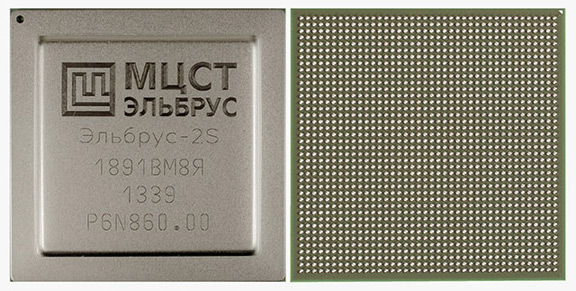
\includegraphics[width=0.7\textwidth]{elbrus-2s}
\end{figure}

\end{frame}

\begin{frame}{Преимущества}
\begin{itemize}
    \item Распределением вычислительных устройств занимается компилятор,
    \item Пониженное энергопотребление, за счет отсуствия узлов, отвечающих за
    распределение задач.
\end{itemize}
\end{frame}

\begin{frame}{Недостатки}
\begin{itemize}
    \item Низкая плотность кода. Большое количество NOP-инструкций,
    \item Увеличенный размер программ,
    \item Сложность программирования на уровне ISA. Только оптимизации
    компилятора.
\end{itemize}
\end{frame}

\begin{frame}{Реализации}
\begin{itemize}
    \item Микропроцессоры серии <<Эльбрус>>,
    \item TriMedia (NXP Semiconductors). 1987--2010 гг.,
    \item Transmeta Crusoe. 2000--2004 гг.
    \begin{figure}[htbp]
        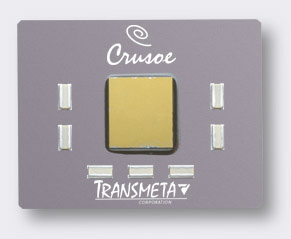
\includegraphics[width=0.4\textwidth]{transmeta-crusoe}
    \end{figure}
\end{itemize}
\end{frame}

\begin{frame}[fragile]{Пример}

Код складывающий 4 числа, находящихся в регистрах R1, R2, R3, R4.

\begin{lstlisting}
R5 = R1 + R2, R6 = R3 + R4;
R0 = R5 + R6, NOP;
\end{lstlisting}

\end{frame}

\section*{Литература}

\begin{frame}[allowframebreaks]{Рекомендуемая литература}
\begin{thebibliography}{99}
    \bibitem{patterson-hennessy} \textit{David A. Patterson, John L. Hennessy}. <<Computer Organization and Design, Fourth Edition: The Hardware/Software Interface.>>
    \bibitem{vliw} <<Introduction to VLIW Computer Architecture>>. // Introduction to VLIW Computer Architecture. \url{http://www.psut.edu.jo/sites/qaralleh/CO/CA Documents/11_vliw.pdf}
\end{thebibliography}
\end{frame}

\section*{Конец}

\begin{frame}{На следующей лекции}
\end{frame}

\begin{frame}

{\huge{Спасибо за внимание!}\par}

\vfill

\tiny{\textit{Замечание}: все торговые марки и логотипы, использованные в данном материале, являются собственностью их владельцев. Представленная здесь точка зрения отражает личное мнение автора, не выступающего от лица какой-либо организации.}

\end{frame}

\end{document}
